% ICVSS poster format (70x90cm); landscape orientation is not allowed
\documentclass[ICVSS,portrait,final]{baposter}
% Generic poster format
%\documentclass[portrait,final]{baposter}
% a4shrink for an a4 sized paper (WARNING: aspect ratio of ICVSS posters is different from A4, may break layout)
%\documentclass[a4shrink,portrait,final]{baposter}

% ABOUT THIS TEMPLATE
% Poster template by Brian Amberg 2007
% Little changes and current ICVSS template by Eugenio Rustico 2010 (rustico@dmi.unict.it)
% Please do not mail us for general LaTeX questions. Thank you!
% Feel free to define new colors, change shape and layout of headerboxes.
% You can add an eyecatcher, set a background image, avoid drawing some headers (ghost option).
% About headerboxes: remember to define first the top and bottom ones.
%
% KNOWN ISSUES
% - Something is wrong with some eyecatchers
% - Using pdftex breaks the page size [partially solved]

% Using pdftex (required by hyperref package) may lead to wrong page size.
% However, there is a workaround to import hyperref without breaking the
% page layout (thanks to Christian Nitschke for pointing it out).
% It is described here:
%   http://stackoverflow.com/questions/1496852/page-margins-change-in-pdflatex/1843929#1843929
% However, for some reasons background shading seems to be lost.
% To summarize: if you *really* need hyperref, choose a plain white background and
% uncomment the following:
% ---------------- FROM HERE
% \setlength{\paperwidth}{700mm}
% \setlength{\paperheight}{900mm}
% if PDFTeX
% % set commands \pdfpagewidth, \pdfpageheight which are only known to PDFTeX
% \ifx\pdfoutput\undefined
% \else
% \setlength{\pdfpagewidth}{\paperwidth}
% \setlength{\pdfpageheight}{\paperheight}
% \fi
% ---------------- TO HERE

\tracingstats=2

% Words in captital letters are marked as acronyms and hyphenated wrong.
% Let's tell LaTeX not to hyphen capitals at all
\uchyph=0

% Euro symbol
\usepackage{eurosym}
% hyperlinks
% can use hyperref (see above), but background shading may be lost (use plain white?)
%\usepackage[colorlinks=true,pdftex]{hyperref}
% urls
\usepackage{url}

\usepackage{times}
\usepackage{calc}
\usepackage{graphicx}
\usepackage{amsmath}
\usepackage{amssymb}
\usepackage{relsize}
\usepackage{multirow}
\usepackage{bm}

\usepackage{graphicx}
\usepackage{multicol}

\usepackage{pgfbaselayers}
\pgfdeclarelayer{background}
\pgfdeclarelayer{foreground}
\pgfsetlayers{background,main,foreground}

\usepackage{helvet}
%\usepackage{bookman}
\usepackage{palatino}

\newcommand{\captionfont}{\footnotesize}

\selectcolormodel{cmyk}

% all imgs in a subdir
\graphicspath{{images/}}

%%%%%%%%%%%%%%%%%%%%%%%%%%%%%%%%%%%%%%%%%%%%%%%%%%%%%%%%%%%%%%%%%%%%%%%%%%%%%%%%
%%%% Some math symbols used in the text
%%%%%%%%%%%%%%%%%%%%%%%%%%%%%%%%%%%%%%%%%%%%%%%%%%%%%%%%%%%%%%%%%%%%%%%%%%%%%%%%
% Format
\newcommand{\Matrix}[1]{\begin{bmatrix} #1 \end{bmatrix}}
\newcommand{\Vector}[1]{\Matrix{#1}}
\newcommand*{\SET}[1]  {\ensuremath{\mathcal{#1}}}
\newcommand*{\MAT}[1]  {\ensuremath{\mathbf{#1}}}
\newcommand*{\VEC}[1]  {\ensuremath{\bm{#1}}}
\newcommand*{\CONST}[1]{\ensuremath{\mathit{#1}}}
\newcommand*{\norm}[1]{\mathopen\| #1 \mathclose\|}% use instead of $\|x\|$
\newcommand*{\abs}[1]{\mathopen| #1 \mathclose|}% use instead of $\|x\|$
\newcommand*{\absLR}[1]{\left| #1 \right|}% use instead of $\|x\|$

\def\norm#1{\mathopen\| #1 \mathclose\|}% use instead of $\|x\|$
\newcommand{\normLR}[1]{\left\| #1 \right\|}% use instead of $\|x\|$

%%%%%%%%%%%%%%%%%%%%%%%%%%%%%%%%%%%%%%%%%%%%%%%%%%%%%%%%%%%%%%%%%%%%%%%%%%%%%%%%
% Multicol Settings
%%%%%%%%%%%%%%%%%%%%%%%%%%%%%%%%%%%%%%%%%%%%%%%%%%%%%%%%%%%%%%%%%%%%%%%%%%%%%%%%
\setlength{\columnsep}{0.7em}
\setlength{\columnseprule}{0mm}

%%%%%%%%%%%%%%%%%%%%%%%%%%%%%%%%%%%%%%%%%%%%%%%%%%%%%%%%%%%%%%%%%%%%%%%%%%%%%%%%
% Save space in lists. Use this after the opening of the list
%%%%%%%%%%%%%%%%%%%%%%%%%%%%%%%%%%%%%%%%%%%%%%%%%%%%%%%%%%%%%%%%%%%%%%%%%%%%%%%%
\newcommand{\compresslist}{%
\setlength{\itemsep}{1pt}%
\setlength{\parskip}{0pt}%
\setlength{\parsep}{0pt}%
}


%%%%%%%%%%%%%%%%%%%%%%%%%%%%%%%%%%%%%%%%%%%%%%%%%%%%%%%%%%%%%%%%%%%%%%%%%%%%%%
%%% Begin of Document
%%%%%%%%%%%%%%%%%%%%%%%%%%%%%%%%%%%%%%%%%%%%%%%%%%%%%%%%%%%%%%%%%%%%%%%%%%%%%%

\begin{document}

%%%%%%%%%%%%%%%%%%%%%%%%%%%%%%%%%%%%%%%%%%%%%%%%%%%%%%%%%%%%%%%%%%%%%%%%%%%%%%
%%% Here starts the poster
%%%---------------------------------------------------------------------------
%%% Format it to your taste with the options
%%%%%%%%%%%%%%%%%%%%%%%%%%%%%%%%%%%%%%%%%%%%%%%%%%%%%%%%%%%%%%%%%%%%%%%%%%%%%%
% Define some colors
\definecolor{silver}{cmyk}{0,0,0,0.3}
\definecolor{yellow}{cmyk}{0,0,0.9,0.0}
\definecolor{reddishyellow}{cmyk}{0,0.22,1.0,0.0}
\definecolor{black}{cmyk}{0,0,0.0,1.0}
\definecolor{darkYellow}{cmyk}{0,0,1.0,0.5}
\definecolor{darkSilver}{cmyk}{0,0,0,0.1}

\definecolor{lightyellow}{cmyk}{0,0,0.3,0.0}
\definecolor{lighteryellow}{cmyk}{0,0,0.1,0.0}
\definecolor{lighteryellow}{cmyk}{0,0,0.1,0.0}
\definecolor{lightestyellow}{cmyk}{0,0,0.05,0.0}

\definecolor{icvss_gray}{cmyk}{0.13,0,0.08,0.56}

\definecolor{icvss_blue}{cmyk}{0.65, 0.24, 0, 0.10}
\definecolor{icvss_darkblue}{RGB}{0,60,120}
\definecolor{icvss_2015}{RGB}{134,124,0}
\definecolor{icvss_lightblue}{RGB}{240,240,255}
\definecolor{icvss_glicine}{RGB}{219,212,255}
%\definecolor{icvss_blue}{RGB}{60,140,190}
%\definecolor{icvss_lblue}{RGB}{100,152,203}
\definecolor{icvss_gray}{RGB}{250,250,250}

\definecolor{iblue}{RGB}{0,0,255}
\definecolor{igray}{RGB}{100,100,100}

%%
\typeout{Poster Starts}

% Background image
%\background{
%  \begin{tikzpicture}[remember picture,overlay]%
%    \draw (current page.north west)+(-2em,2em) node[anchor=north west] {\includegraphics[height=1.1\textheight]{file_background}};
%  \end{tikzpicture}%
%}

\newlength{\leftimgwidth}

%\rule{\textwidth}{1pt}
\begin{poster}%
  % Poster Options
  {
  % Show grid to help with alignment
  grid=no,
  % Column spacing
  colspacing=1em,
  % Color style
  bgColorOne=white,
    %bgColorTwo=lightgray,
    bgColorTwo=white,
  %borderColor=icvss_darkblue,
  borderColor=black,
    headerColorOne=icvss_2015,
    %headerColorOne=icvss_glicine,
    %headerColorOne=icvss_blue,
  %headerColorTwo=icvss_blue,
  headerColorTwo=white,
    headerFontColor=white,
    %headerFontColor=black,
  boxColorOne=white,
  boxColorTwo=icvss_gray,
  % Format of textbox
  textborder=roundedleft,
  % Format of text header
  eyecatcher=no,
  headerborder=closed,
  headerheight=0.10\textheight,
  headershape=roundedright,
    headershade=shade-lr,
    %headershade=plain,
  headerfont=\Large\textsf, %Sans Serif
  % Shading
    boxshade=shade-tb,
    % boxshade=plain,
  %background=plain,
  background=shade-tb,
  linewidth=1pt
  }

  % Eye Catcher
  %{ \includegraphics[width=10em]{D1077} % No eye catcher for this poster. (eyecatcher=no above). If an eye catcher is present, the title is centered between eye-catcher and logo.
   %}
  % Title
  {\sf %Sans Serif
  %\bf% Serif
  \vspace{0.5em}
  % may be one- or two-rows
  TACKLING BACKGROUND DIFFERENTLY\\
%   \LaTeX ~ POSTER TEMPLATE
  }
  % Authors
  {\sf %Sans Serif
  % Serif
  \begin{normalsize}Jetley S., Romera-Paredes B., Torr P. - University of
  Oxford\\
  \vspace{0.4em}\{sjetley, bernard, phst\}@robots.ox.ac.uk
  \end{normalsize}
  }
  % University logo
  % The makebox allows the title to flow into the logo, this is a hack because of the L shaped logo.
  {
    \makebox[10em][r]{%
      \begin{minipage}{18em} % short logo version
      %\begin{minipage}{\textwidth} % long log version
        %\hfill
        % don't want logo to stick to the document edge
        %\advance\leftskip-6em
        \hspace*{-9em}
        %\includegraphics[height=6em]{icvsslogo} % short logo version
        \begin{flushright}
        
\includegraphics[height=4em]{Logo_2015.jpg} % B/W logo version
        \end{flushright}
      \end{minipage}
    }
}

  \tikzstyle{light shaded}=[top color=baposterBGtwo!30!white,bottom color=baposterBGone!30!white,shading=axis,shading angle=30]

  % Width of left inset image
     \setlength{\leftimgwidth}{0.78em+8.0em}

%%%%%%%%%%%%%%%%%%%%%%%%%%%%%%%%%%%%%%%%%%%%%%%%%%%%%%%%%%%%%%%%%%%%%%%%%%%%%%
%%% Now define the boxes that make up the poster
%%%---------------------------------------------------------------------------
%%% Each box has a name and can be placed absolutely or relatively.
%%% The only inconvenience is that you can only specify a relative position
%%% towards an already declared box. So if you have a box attached to the
%%% bottom, one to the top and a third one which should be in between, you
%%% have to specify the top and bottom boxes before you specify the middle
%%% box.
%%%%%%%%%%%%%%%%%%%%%%%%%%%%%%%%%%%%%%%%%%%%%%%%%%%%%%%%%%%%%%%%%%%%%%%%%%%%%%
    %
    % A coloured circle useful as a bullet with an adjustably strong filling
    \newcommand{\colouredcircle}[1]{c%
      \tikz{\useasboundingbox (-0.2em,-0.32em) rectangle(0.2em,0.32em);
      \draw[draw=black,fill=baposterBGone!80!black!#1!white,line width=0.03em] (0,0) circle(0.18em); }
      }

%%%%%%%%%%%%%%%%%%%%%%%%%%%%%%%%%%%%%%%%%%%%%%%%%%%%%%%%%%%%%%%%%%%%%%%%%%%%%%
\headerbox{Abstract}{name=abstract,column=0,row=0,span=1.25}{
%%%%%%%%%%%%%%%%%%%%%%%%%%%%%%%%%%%%%%%%%%%%%%%%%%%%%%%%%%%%%%%%%%%%%%%%%%%%%%
%\smaller
Practical vision systems need to identify objects from amongst $n$
different classes of interest while distinguishing them from the residual
image content i.e. the background. Background does not have one
consistent definition, yet highly successful approaches based on
CNNs\cite{RCNN,FCN}, treat it as a regular object category and attempt to learn
its appearance. This is counter-intuitive.

We propose a modified deepnet architecture for tackling background class as
'something other than the objects of interest'. We filter the background samples 
using a threshold that is learnt via end-to-end training and not as an optimum
of a sub-problem. Separating the background samples allows us to define unambiguous
output embedding space for just the object classes which offers	 a promising
potential to boost classification as well as zero-shot performance.
}

%%%%%%%%%%%%%%%%%%%%%%%%%%%%%%%%%%%%%%%%%%%%%%%%%%%%%%%%%%%%%%%%%%%%%%%%%%%%%%
 \headerbox{Motivation}{name=motivation,column=1.25,span=1.8}{
%%%%%%%%%%%%%%%%%%%%%%%%%%%%%%%%%%%%%%%%%%%%%%%%%%%%%%%%%%%%%%%%%%%%%%%%%%%%%%
Issues with the traditional way of handling 'background' in a deepnet:
\begin{itemize}
\item Learning \textbf{dissimilar visual patterns} as background class is
counter-intuitive
\item Priors such as \textbf{natural language semantics, attributes are not available} for background class
\end{itemize}
%   \vspace{0.3em}
}

%%%%%%%%%%%%%%%%%%%%%%%%%%%%%%%%%%%%%%%%%%%%%%%%%%%%%%%%%%%%%%%%%%%%%%%%%%%%%%
 \headerbox{ProposedApproach}{name=proapp,column=1.25,below=motivation,span=1.8}{
 The aim is to describe the background class with a threshold T (fixed or
 learned), such that:
\begin{center}
$x$ =
\begin{cases}
${\rm background}$, & \text{if }  $s_c$ < $T$ \forall\text{ }c
\in\{1,\ldots,C\}\\
${\rm object}$, & \text{otherwise}
\end{cases}
\end{center}
, where $x$ is the input sample and $s_c$ is the score (activation) before the
final softmax layer and $C$ is the total number of object classes (ref. Fig.1).
}
%%%%%%%%%%%%%%%%%%%%%%%%%%%%%%%%%%%%%%%%%%%%%%%%%%%%%%%%%%%%%%%%%%%%%%%%%%%%%%
%%%%%%%%%%%%%%%%%%%%%%%%%%%%%%%%%%%%%%%%%%%%%%%%%%%%%%%%%%%%%%%%%%%%%%%%%%%%%%
\headerbox{References}{name=references,column=0,span=2,above=bottom}{
%%%%%%%%%%%%%%%%%%%%%%%%%%%%%%%%%%%%%%%%%%%%%%%%%%%%%%%%%%%%%%%%%%%%%%%%%%%%%%
    \smaller
    \vspace{-0.4em}
    \bibliographystyle{ieee}
    \renewcommand{\section}[2]{\vskip 0.05em}
      \begin{thebibliography}{1}\itemsep=-0.01em
	\setlength{\baselineskip}{0.4em}
	\bibitem{RCNN}
	  Ren, Shaoqing, et al. "Faster R-CNN: Towards Real-Time Object Detection with
	  Region Proposal Networks." arXiv:1506.01497 (2015).
	\bibitem{FCN}
	 Long, Jonathan, Evan Shelhamer, and Trevor Darrell. "Fully convolutional networks for semantic segmentation." arXiv:1411.4038 (2014).
    \bibitem{proto}
	 Jetley, Saumya, et al. "Prototypical Priors: From Improving Classification to Zero-Shot Learning." BMVC. 2015.
    \end{thebibliography}
  }
% 
%%%%%%%%%%%%%%%%%%%%%%%%%%%%%%%%%%%%%%%%%%%%%%%%%%%%%%%%%%%%%%%%%%%%%%%%%%%%%%
  \headerbox{Proposed
  Architecture}{name=pro_archi,column=0,span=2,below=abstract}{
%%%%%%%%%%%%%%%%%%%%%%%%%%%%%%%%%%%%%%%%%%%%%%%%%%%%%%%%%%%%%%%%%%%%%%%%%%%%%%
\begin{center}
  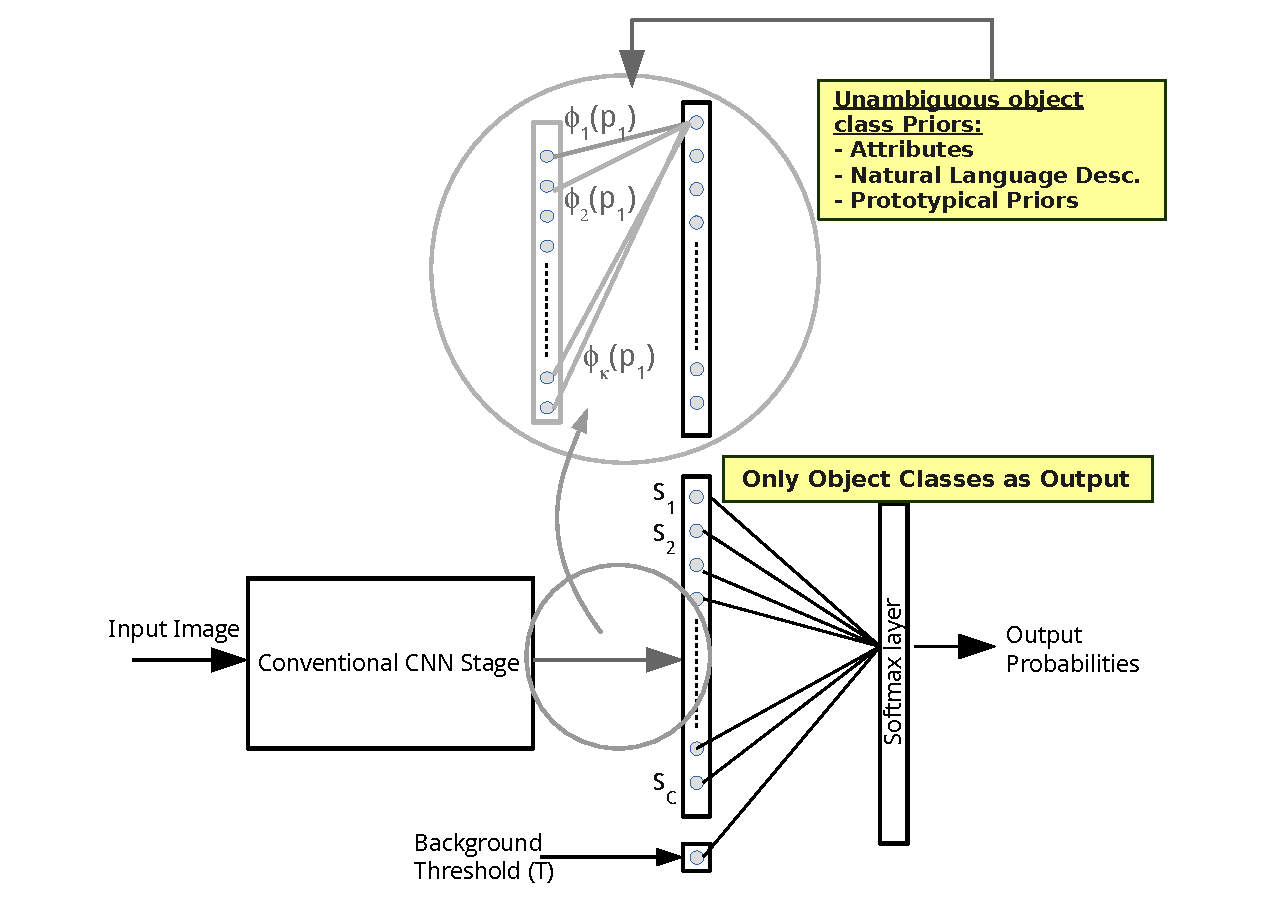
\includegraphics[height=27.5em]{images/poster_icvss_re-final1.pdf}
\end{center}
}

%%%%%%%%%%%%%%%%%%%%%%%%%%%%%%%%%%%%%%%%%%%%%%%%%%%%%%%%%%%%%%%%%%%%%%%%%%%%%%
  \headerbox{Benefits}{name=benefits,column=2,span=1.05,below=proapp}{
%%%%%%%%%%%%%%%%%%%%%%%%%%%%%%%%%%%%%%%%%%%%%%%%%%%%%%%%%%%%%%%%%%%%%%%%%%%%%%
\begin{itemize}
  \item Background is intuitively treated as an entity other than the objects
  of interest, for which \textbf{object class activation is < $T$}
  \item Allows \textbf{end-to-end learning} of background threshold
  \item \textbf{Unambiguous class priors} such as natural language semantics or
  visual attributes can be leveraged in end-to-end training \cite{proto}
  \textbf{as the set of fixed weights $\phi$ }(Ref. Fig.1)
\end{itemize}
  }
%%%%%%%%%%%%%%%%%%%%%%%%%%%%%%%%%%%%%%%%%%%%%%%%%%%%%%%%%%%%%%%%%%%%%%%%%%%%%%
  \headerbox{Dataset}{name=dataset,column=2,span=1.05,below=benefits}{
%%%%%%%%%%%%%%%%%%%%%%%%%%%%%%%%%%%%%%%%%%%%%%%%%%%%%%%%%%%%%%%%%%%%%%%%%%%%%%
German Traffic Sign Dataset (43 classes):
%\begin{itemize}

 \textbf{Training}: 39209 object samples \& 1410 background samples

 \textbf{Val \& Test}: 6316 object samples \& 450 background samples;
  6315 object samples \& 525 background samples
%\end{itemize}
}

%%%%%%%%%%%%%%%%%%%%%%%%%%%%%%%%%%%%%%%%%%%%%%%%%%%%%%%%%%%%%%%%%%%%%%%%%%%%%%
  \headerbox{Results}{name=results,column=2,span=1.05,below=dataset}{
%%%%%%%%%%%%%%%%%%%%%%%%%%%%%%%%%%%%%%%%%%%%%%%%%%%%%%%%%%%%%%%%%%%%%%%%%%%%%%
\textbf{Results are promising}:
\begin{center}
\begin{tabular}{|c|c|}
\hline 
%Description & \shortstack{Test\\Accuracy (\%)}\tabularnewline
Description & Test Acc.(\%)\tabularnewline
\hline 
\hline 
\shortstack{Background \\ as object} & 95.77\tabularnewline
\hline 
Fixed-T & 95.19\tabularnewline
\hline 
Learned-T & 95.68\tabularnewline
\hline 
\end{tabular}
\end{center}
}

% %%%%%%%%%%%%%%%%%%%%%%%%%%%%%%%%%%%%%%%%%%%%%%%%%%%%%%%%%%%%%%%%%%%%%%%%%%%%%%
%   \headerbox{Scholarship}{name=scholarship,column=2,row=0}{
% %%%%%%%%%%%%%%%%%%%%%%%%%%%%%%%%%%%%%%%%%%%%%%%%%%%%%%%%%%%%%%%%%%%%%%%%%%%%%%
% A scholarship of 500\euro~(grant offered by GIRPR)
% will be awarded to
% the best PhD student attending the school. The decision will be made by the
% School Committee at the time of the School, taking into account candidates'cv,
% poster and oral presentation. All PhD students attending the school will be
% considered for the ICVSS grant.
% 
% \begin{center}
%   
\includegraphics[width=0.6\linewidth]{GIRinPR.jpg}
% \end{center}
%   \vspace{0.3em}
%   }
% 
% 
% 
% %%%%%%%%%%%%%%%%%%%%%%%%%%%%%%%%%%%%%%%%%%%%%%%%%%%%%%%%%%%%%%%%%%%%%%%%%%%%%%
% %\headerbox{Poster}{name=poster,column=1,span=2,below=scholarship,above=acknowledge,ghost=yes}{
% \headerbox{Poster}{name=poster,column=1,span=2,below=scholarship,above=acknowledge}{
% %%%%%%%%%%%%%%%%%%%%%%%%%%%%%%%%%%%%%%%%%%%%%%%%%%%%%%%%%%%%%%%%%%%%%%%%%%%%%%
% The poster should be written in English and should be sent (See Poster Submission section \cite{submissionlink})
% in a printable pdf format. For your poster, a board will be provided which
% measures $90\times70~\mbox{cm}$.
% 
% \begin{center}
%   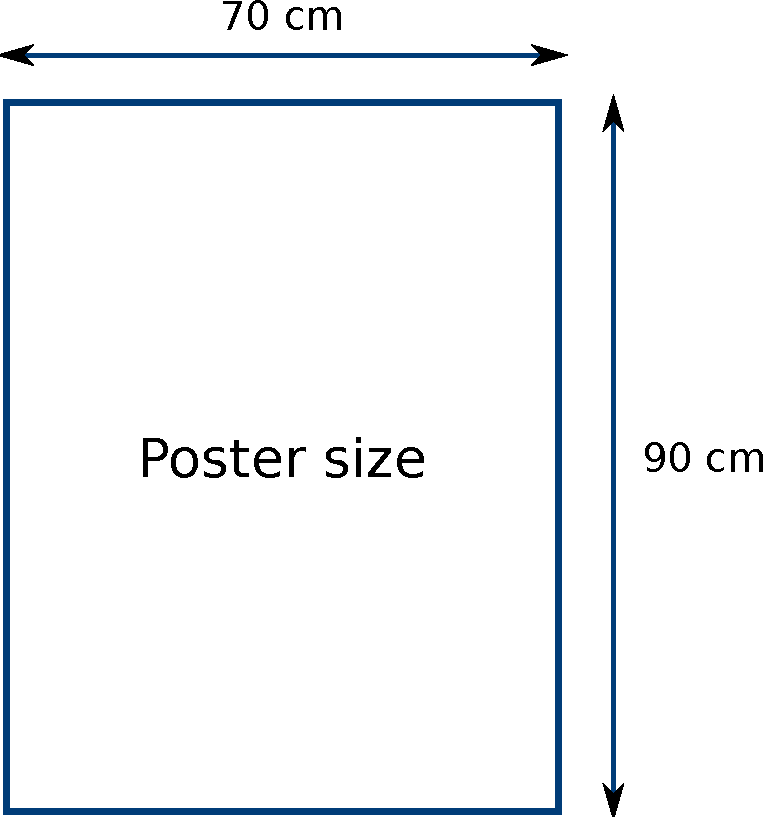
\includegraphics[width=0.5\linewidth]{postersize}
% \end{center}
% 
% You need to print and bring with you the poster
% to the school. Push tacks or velcro adhesive will be provided at the conference
% to mount your poster to the board. Submission not satisfying the guidelines will
% be rejected \cite{calllink}.
% 
% 
%   \vspace{0.3em}
%   }
% 
% %%%%%%%%%%%%%%%%%%%%%%%%%%%%%%%%%%%%%%%%%%%%%%%%%%%%%%%%%%%%%%%%%%%%%%%%%%%%%%
%   \headerbox{Best Presentation Prize}{name=prize,column=1,row=0,above=poster}{
% %%%%%%%%%%%%%%%%%%%%%%%%%%%%%%%%%%%%%%%%%%%%%%%%%%%%%%%%%%%%%%%%%%%%%%%%%%%%%%
% A selected subset from the submitted posters will be selected by the school committee
% for short oral presentation. A best presentation prize of 500\euro~ (supported by Toshiba
% Research Europe) will be given to the best presentation selected by the school committee.
% Notification for oral presentation will be given by 17 July 2015 (same day of the presentation).
%   %\vspace{3em}
% \begin{center}
%   
\includegraphics[width=0.72\linewidth]{toshiba_logo}
% \end{center}
% \vspace{0.3em}
%   }

%%%%%%%%%%%%%%%%%%%%%%%%%%%%%%%%%%%%%%%%%%%%%%%%%%%%%%%%%%%%%%%%%%%%%%%%%%%%%%
\end{poster}

\end{document}
